\section{Method}
\label{sect:method}

This section presents our  method TF design, which enables semi-automated material classification and initial TF definition to support intuitive volume exploration.

An overview is presented in Fig.~\ref{fig:volume-exploration-pipeline}. After organizing the multidimensional data into a volume grid, our method comprises three main steps: dimensionality reduction, clustering and representative selection.

The techniques employed at each step were carefully chosen based on their computational complexity, ensuring a balance between efficiency and effectiveness when handling large volume datasets. This design supports practical scalability and responsiveness, which are critical for interactive exploration.

\begin{figure*}[htb!]
    \centering
    \caption{Overview of the proposed transfer function design.}
    \label{fig:volume-exploration-pipeline}
    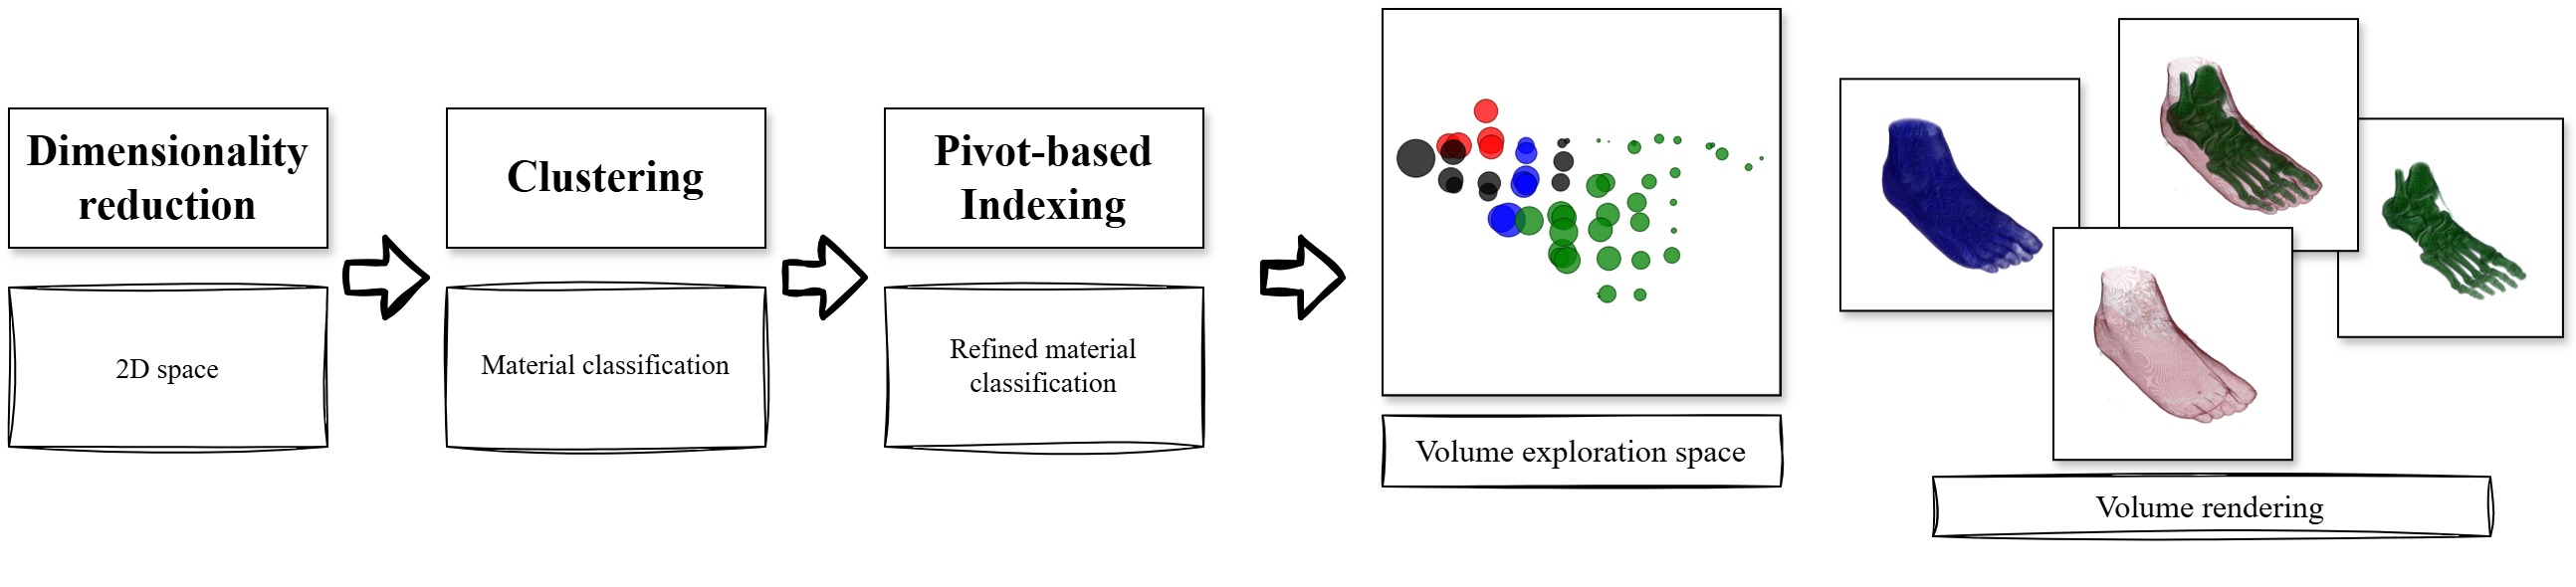
\includegraphics[width=\textwidth]{figs/method-overview.jpg}
\end{figure*}

\subsection{Dimensionality reduction}
\label{subsect:feature-extraction}

Dimensionality reduction is a critical step for two reasons. First, the clustering technique employed requires a two-dimensional input space for proper functioning (see Section~\ref{subsect:clustering}). Second, our TF design interface is inherently two-dimensional (see Section~\ref{sect:volume-exploration}).

We adopt FastMap~\cite{faloutsos1995} to project high-dimensional voxel data into a 2D space while preserving data similarity. FastMap operates by selecting two distant pivots and projecting all points onto the line defined by these pivots, recursively reducing the dimensionality.

Let $d$ be the number of attributes and $n$ the number of voxels. The algorithm proceeds as follows:

\begin{enumerate}
    \item Select two points with maximal pairwise distance as the pivots.
    \item Project all points onto a hyperplane orthogonal to the line defined by the pivots.
\end{enumerate}

To mitigate the computational cost of pivot selection, \citet{faloutsos1995} proposed the approach summarized in Algorithm~\ref{alg:pivot-searching-of-fastmap}.

\begin{algorithm}
    \caption{Pivot searching in FastMap.}
    \label{alg:pivot-searching-of-fastmap}
    \KwIn{$\mathbb{O}$}
    \KwOut{Pivots $O_a$, $O_b$}
    $O_a \gets$ random point $o \in \mathbb{O}$\\
    $O_b \gets$ point $o \in \mathbb{O}$ farthest from $O_a$\\
    $O_a \gets$ point $o \in \mathbb{O}$ farthest from $O_b$
\end{algorithm}

\subsection{Clustering}
\label{subsect:clustering}

To simplify material classification and enhance the detection of relevant volume structures, we employ the classical density-based clustering technique DBSCAN~\cite{ester1996}.

DBSCAN is widely recognized for its ability to detect clusters of arbitrary shape without requiring prior knowledge of the number of clusters~\cite{schubert2017}. However, its standard implementation has a worst-case time complexity of $\mathcal{O}(n^2)$~\cite{schubert2017}. To ensure practical scalability, we adopt an optimized grid-based variant~\cite{gunawan2013}, which reduces the time complexity to $\mathcal{O}(n \log n)$.

As in the original algorithm, two parameters must be tuned by the user: $minPts$, the minimum number of points to form a dense region, and $\varepsilon$, the neighborhood radius.

At the end of this step, each cluster contains a subset of voxels potentially representing distinct FOI within the volume.

\subsection{Representative selection}
\label{subsect:representative-selection}

The voxels classified by DBSCAN could be directly projected onto the TF design interface. However, to reduce clutter in the scatter plot and improve interpretability, we apply a representative selection technique within each cluster.

First, representative pivots are selected using Sparse Spatial Selection (SSS)~\cite{pedreira2007}. This technique iteratively adds points as pivots if they are sufficiently distant from all previously selected pivots, with the distance controlled by a factor $\alpha$ (Algorithm~\ref{alg:sss}).

\begin{algorithm}
    \caption{Sparse Spatial Selection (SSS).}
    \label{alg:sss}
    \KwIn{Points $\mathbb{P}$}
    \KwOut{Selected pivots $\mathbb{P}_s$}
    $\mathbb{P}_s \gets \{p_1\}$ \\
    \ForEach{$p \in \mathbb{P}$}{
        \If{$\forall p_s \in \mathbb{P}_s, \text{dist}(p, p_s) \geq M\alpha$}{
            $\mathbb{P}_s \gets \mathbb{P}_s \cup \{p\}$
        }
    }
\end{algorithm}

Next, each cluster is subdivided into sub-clusters by assigning every point to its nearest pivot (Algorithm~\ref{alg:subclustering-finding}). This step refines the initial classification and acts as a second-level clustering, improving the granularity of FOI representation.

\begin{algorithm}
    \caption{Sub-cluster assignment within a cluster.}
    \label{alg:subclustering-finding}
    \KwIn{Points $\mathbb{P}$ of cluster $c$}
    \KwIn{Pivots $\mathbb{P}_s$ of cluster $c$}
    \KwOut{Points with sub-cluster assignments}
    \ForEach{$p \in \mathbb{P}$}{
        $p_s \gets$ nearest pivot in $\mathbb{P}_s$ \\
        Assign $p$ to $p_s$'s sub-cluster
    }
\end{algorithm}

The parameter $\alpha$ controls the number of selected pivots: smaller values lead to more pivots and finer sub-clustering, while values closer to $1$ yield fewer, broader sub-clusters.
